\chapter{Generative Adversarial Networks : Principles, strengths and limitations}
\label{chap:chapter1}

\begin{chapterabstract}
	In this chapter, we propose an overview	 of the Generative Adversarial Networks \cite{Goodfellow2014} framework, some of its theoretical interpretations, as well as some of its variations and applications. We discuss the different limitations of this approach and expose a trilemma between the quality of the generated samples, their diversity and the conditioning of the model. We then discuss the recent advances that have been made to overcome some of these limitations and propose a classification of these advances using the aforementioned trilemma. Finally, we discuss the evaluation of generative models and the difficulties of evaluating the intrinsic quality of a generated sample.  We propose an overview of the different classical metrics and discuss their limitations.
\end{chapterabstract}

\minitoc

\section{Generative Adversarial Networks}

<<<<<<< HEAD
In this section, we introduce the Generative Adversarial Networks \cite{Goodfellow2014}.  We will first 

\subsection{The GAN framework}

GAN formulation, loss variations, JS/KL interpretation of the loss

\subsection{Conditional modeling with  \ac{GAN}}
=======
Generative Adversarial Networks (\ac{GAN}) \cite{Goodfellow2014} have been recently highlighted for their ability to generate photo-realistic images.

\subsection{Deep generative modeling}

Generative modeling with deep neural networks has been a challenging task due to its fundamentally stochastic nature, which prevents the computation of gradients. Indeed, whereas a discrimination tries to predict the class $y$ of a sample $x \sim \px$, which is to model the conditional probability distribution $\pyx$, the purpose of a generative model is to provide a sampling mechanism over $\px$  the intrinsic distribution of the data. By nature, this sampling mechanism is stochastic and therefore cannot be directly learned through gradient descent.

To overcome this problem,  Generative Stochastic Networks\cite{Bengio2012b}  model instead a parameterized Markov chain which converges to a point of the learned distribution. It uses the ergodicity property to generate samples by consecutive sampling on a randomly chosen starting point. \CR{To extend}

Instead of directly modeling $\px$, Variational Auto-Encoders (\ac{VAE})\cite{Kingmaa} learns to model a deterministic mapping $\pgxz$. From this mapping, the generative model can be obtain through marginalization: $\pgx = \int \pz \pgxz dz$. It then defines a variational lower bound of the data likelihood and trains the model as an auto-encoder which inner representation is pushed towards being the parameters of a Gaussian distribution. To generate a sample from the trained model, a random vector is be sampled from this Gaussian distribution and mapped to the learned distribution by the decoder network.

\CR{Maybe add autoregressive models and flow-based models}

\subsection{The GAN framework}

In the same fashion, Generative Adversarial Networks aims to learn a parameterized mapping $\pgxz$ between a simple distribution $\pz$ (usually normal or uniform) to the real data distribution $\px$. However, instead of trying to estimate the distribution through marginalization, it minimizes an estimation of a divergence between $\px$ and the mapped distribution $\pgx$. 

However, because divergences are usually intractable, \ac{GAN}s rely on a second learned function: the discriminator $\D$.  The discriminator is a binary classifier that learns to distinguish a real sample $x$ from a sample $\G(z)$ generated from $z\sim\pz$ by minimizing the binary cross-entropy. The objective of the generator $\G$ is then to maximize the discriminator's loss. This training process is summed up in the following mini-max game

\begin{equation}
\label{eq:GAN_problem}
\arg\min_\G\max_\D\lgan = \arg\min_G\max_\D \esp_{x\sim \px} [\log \D(x)]  \esp_{z\sim\pz} [1 - \log \D(\G(z))]
\end{equation}

We can show that minimizing the criterion $C( \G) = \max_\D\lgan(D, G)$ is equivalent to minimizing the Jensen-Shannon (\ac{JS}) divergence between $\px$ and $\pgx$\cite{Goodfellow2014}: since the minimum of $f(x) = a\log(x) + b\log(1-x)$ is $\frac{a}{a+b}$, the discriminator that maximizes the criterion for a fixed $\G$ is given by

\begin{equation}
\D^*_\G(x) = \frac{\px}{\px + \pgx}
\end{equation}

By plugin this optimal discriminator in \citeq{eq:GAN_problem}, we get

\begin{align}
		C( \G) &= \max_\D\lgan(D, G) \nonumber\\
		& = \esp_{x\sim \px} \Big[\log \D^*(x)] +  \esp_{z\sim P_z} \Big[1 - \log \D^*(\G(z))\Big] \nonumber = \esp_{x\sim \px} \Big[\log \D^*(x)\Big] +  \esp_{{x}\sim \pgx} \Big[1 - \log \D^*(x)\Big] \nonumber \\
		& = \esp_{x\sim \px} \Big[\log \frac{\px}{\px + \pgx}\Big] +   \esp_{{x}\sim \pgx} \Big[1 - \log  \frac{\pgx}{\px + \pgx}\Big] \nonumber \\
\end{align}

Up to additive and multiplicative constants, the criterion  $C(\G)$ can be reformulated as

\begin{equation}
		C(\G) = \DKL \Big(\px\Big|\Big|\frac{\px+\pgx}{2} \Big) + \DKL \Big(\pgx \Big|\Big| \frac{\px+\pgx}{2} \Big) = 2\cdot\JSD \Big(\px\Big|\Big|\pgx \Big)
\end{equation}

GAN formulation, loss variations, JS/KL interpretation of the loss

\subsection{Conditional modeling with  \ac{GAN}s}
>>>>>>> working
Conditional GANs

Introduction to domain-transfer (Pix2Pix, CycleGAN) through removal of the random noise

\section{Limitations}

Image quality : Incremental enhancement through architecture, more data, ... 

Instability, catastrophic forgetting and the mode collapse problem

Trade-off image quality/diversity : Explanation through the loss term and distribution coverage

Black-box approach to conditioning, no tuning possible, no interpretability

\section{The GAN Zoo}

\subsection{A taxonomy of GANs}
Enorme nombre de variantes de GANs

Taxonomie des approches GANs (pour s'éviter une liste des différents GANs)

Schéma pour définir les grandes familles de GAN (évoquer les AmbientGAN / UNIR)

\subsection{Architecture variants}

\subsection{Divergence variants}
Table des loss alternatives (f-divergences + transport optimal)

\subsection{Task-specific losses}

\begin{figure}
	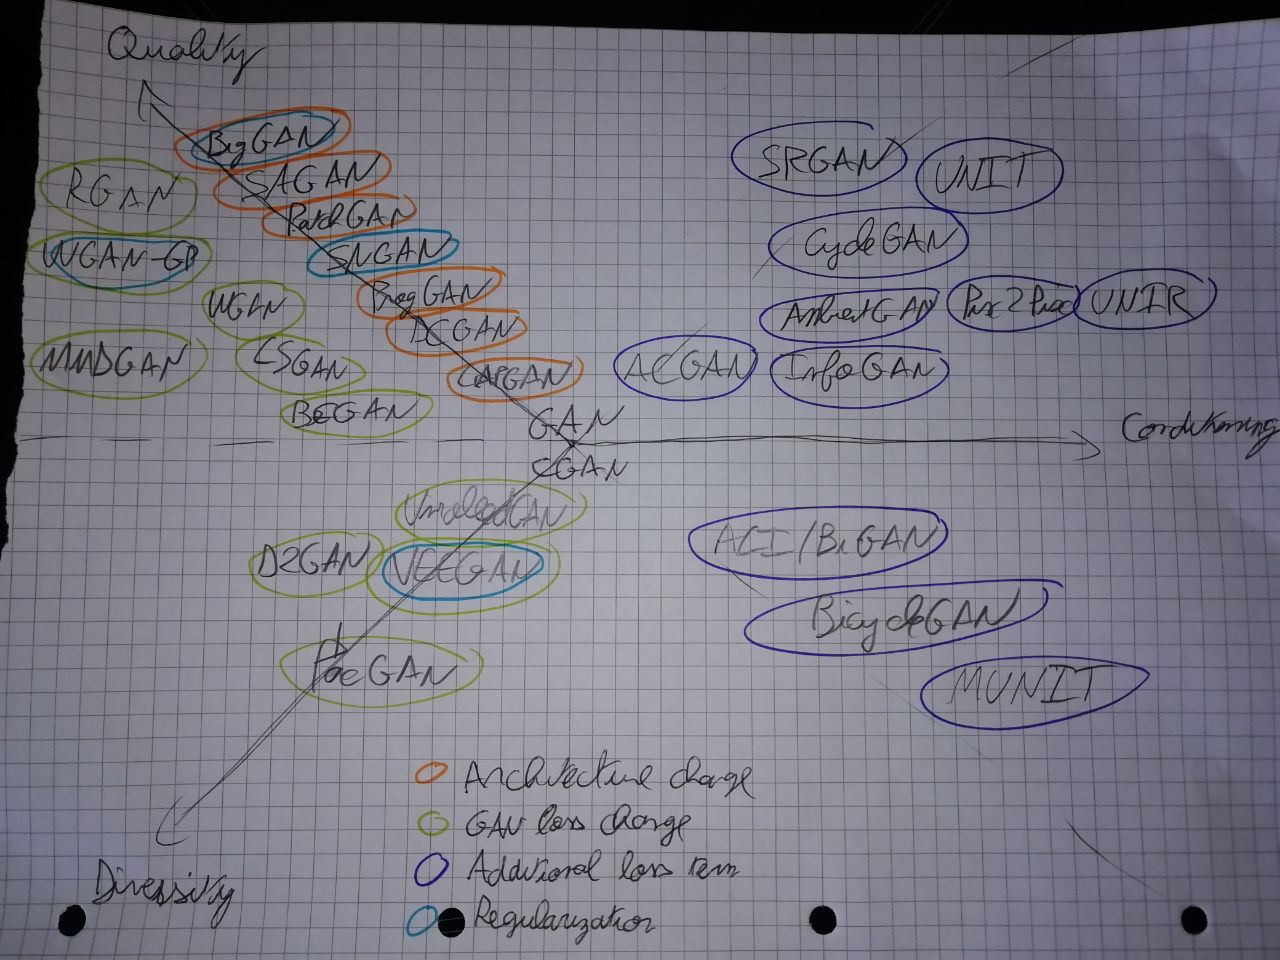
\includegraphics[width=\textwidth]{chapter1/trilemma.jpg}
	\caption{Classifications of some advances in GANs on the trilemma}
\end{figure}

\section{A note on the  evaluation of generative models}

No good adhoc methods

Image quality : Inception distance + Fréchet inception distance, advantages

Conditioning : Direct evaluation (pixel-wise), Classifier accuracy, Projections (PCA, t-SNE)

Limitations of those metrics : need a pre-trained model


